\documentclass{standalone}
\usepackage{tikz}
\usepackage{ctex,siunitx,ninecolors}
\setCJKmainfont{Noto Serif CJK SC}
\usepackage{tkz-euclide}
\usepackage{amsmath}
\usepackage{wasysym}
\usetikzlibrary{patterns, calc}
\usetikzlibrary {decorations.pathmorphing, decorations.pathreplacing, decorations.shapes,}
\begin{document}
\small
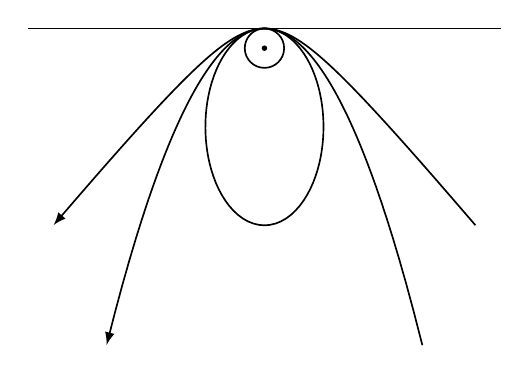
\begin{tikzpicture}[>=latex,scale=1,rotate=-90]
  \draw [domain=0:360,samples=200,semithick] plot (\x:{0.45/(1-0.8*cos(\x))});
  \draw [->,domain=28:332,samples=200,semithick] plot (\x:{0.5/(1-cos(\x))});
  \draw [->,domain=50:310,samples=200,semithick] plot (\x:{0.575/(1-1.3*cos(\x))});
  \draw[semithick](0,0)circle(0.25);
  \draw(-0.25,-3)--(-0.25,3);
  \fill (0,0)circle(1pt);
\end{tikzpicture}
\end{document}
